%!TEX root = ../mieic.tex

\chapter{Projeto}
\label{chap:chap3}

\section*{}

O principal objetivo desta dissertação, como foi referido no capítulo \ref{chap:intro}, é desenvolver um (ou mais) módulo(s) de software que contribuam para uma melhoria na descoberta e recomendação de música num ambiente integrado entre o RAMA e o Spotify, por forma a tirar partido da representação gráfica do grafo de artistas de música do RAMA e da qualidade do serviço de \emph{Streaming} de música do Spotify.

Para tal, a proposta inicial desta dissertação consiste em desenvolver, no mínimo, um módulo que implemente uma das seguintes funcionalidades:

\begin{enumerate}
  \item \label{item:obj1} Integrar o serviço de \emph{streaming} de música do Spotify \textbf{no RAMA}
  \item \label{item:obj2} Integrar informação de um utilizador Spotify \textbf{no RAMA}
  \item \label{item:obj3} Melhorar design e funcionalidades \textbf{do RAMA}
  \item \label{item:obj4} Integrar a visualização de grafos de artistas de música \textbf{numa Aplicação Spotify}
  \item \label{item:obj5} Integrar o módulo de criação de \emph{playlists} do RAMA \textbf{numa Aplicação Spotify}
  \item \label{item:obj6} Integrar alguns dos módulos acima referidos \textbf{numa aplicação móvel}
\end{enumerate}

As três primeiras funcionalidades (\ref{item:obj1}, \ref{item:obj2} e \ref{item:obj3}) focam-se em melhorar o serviço do RAMA, usando API's do Spotify, ou seja, integrar o Spotify dentro do RAMA.
Por outro lado, as funcionalidades \ref{item:obj4} e \ref{item:obj5} têm como objetivo integrar o RAMA dentro do Spotify, através de uma Aplicação Spotify, que funciona como plugin do programa principal do Spotify.
A última funcionalidade (\ref{item:obj6}) teria de implementar algumas das anteriores num Sistema Operativo Móvel (Android, iOS ou Windows Phone).

Este capítulo procura analisar todas as condicionantes que afetam a escolha  dos módulos a desenvolver, e em que ambientes estes se encaixam melhor (Aplicação Spotify, aplicação móvel ou RAMA).

Inicialmente será explorado o ambiente de desenvolvimento que o Spotify disponibiliza, ou seja, que tecnologias tem disponíveis para \emph{developers}.
De seguida serão analisadas quais dessas tecnologias assentam melhor em cada um dos módulos propostos a desenvolver, através de experimentações feitas, e quando necessário, será descrito um possível esquema de arquitetura por forma a facilitar a explicação do problema.


No final deste capítulo, deve ficar claro quais serão os módulos de software a desenvolver, que tecnologias irão ser usadas e qual o esquema geral da sua arquitetura.
O produto final deve de ir ao encontro do objetivo de contribuir para uma melhoria na descoberta e recomendação de música num ambiente relacionado com o RAMA.


\section{Spotify} % (fold)
\label{sec:spotify}

  O Spotify é um serviço de \emph{streaming} de música que permite ouvir, através de uma ligação de Internet, qualquer música que o Spotify possua no seu catálogo.


  \subsection{Ferramentas de Desenvolvimento} % (fold)
  \label{sub:ferramentas_de_desenvolvimento}
  
    No momento de escrita deste relatório, o Spotify tem disponível um conjunto de ferramentas\footnote{http://developer.spotify.com/technologies} para desenvolver módulos de software que podem estar embebidos nas mais diversas aplicações (\emph{third-party applications}) ou então dentro do \emph{Spotify Desktop Client}.

    Existem quatro ferramentas de desenvolvimento, cada uma delas com o seu propósito e utilidade.


    \subsubsection{Spotify Apps} % (fold)
    \label{ssub:spotify_apps}
      Serve para desenvolver Aplicações Spotify\footnote{https://developer.spotify.com/technologies/apps} que são usadas pelos utilizadores Spotify dentro do \emph{Spotify Desktop Client}.

      \begin{figure}
        \begin{center}
          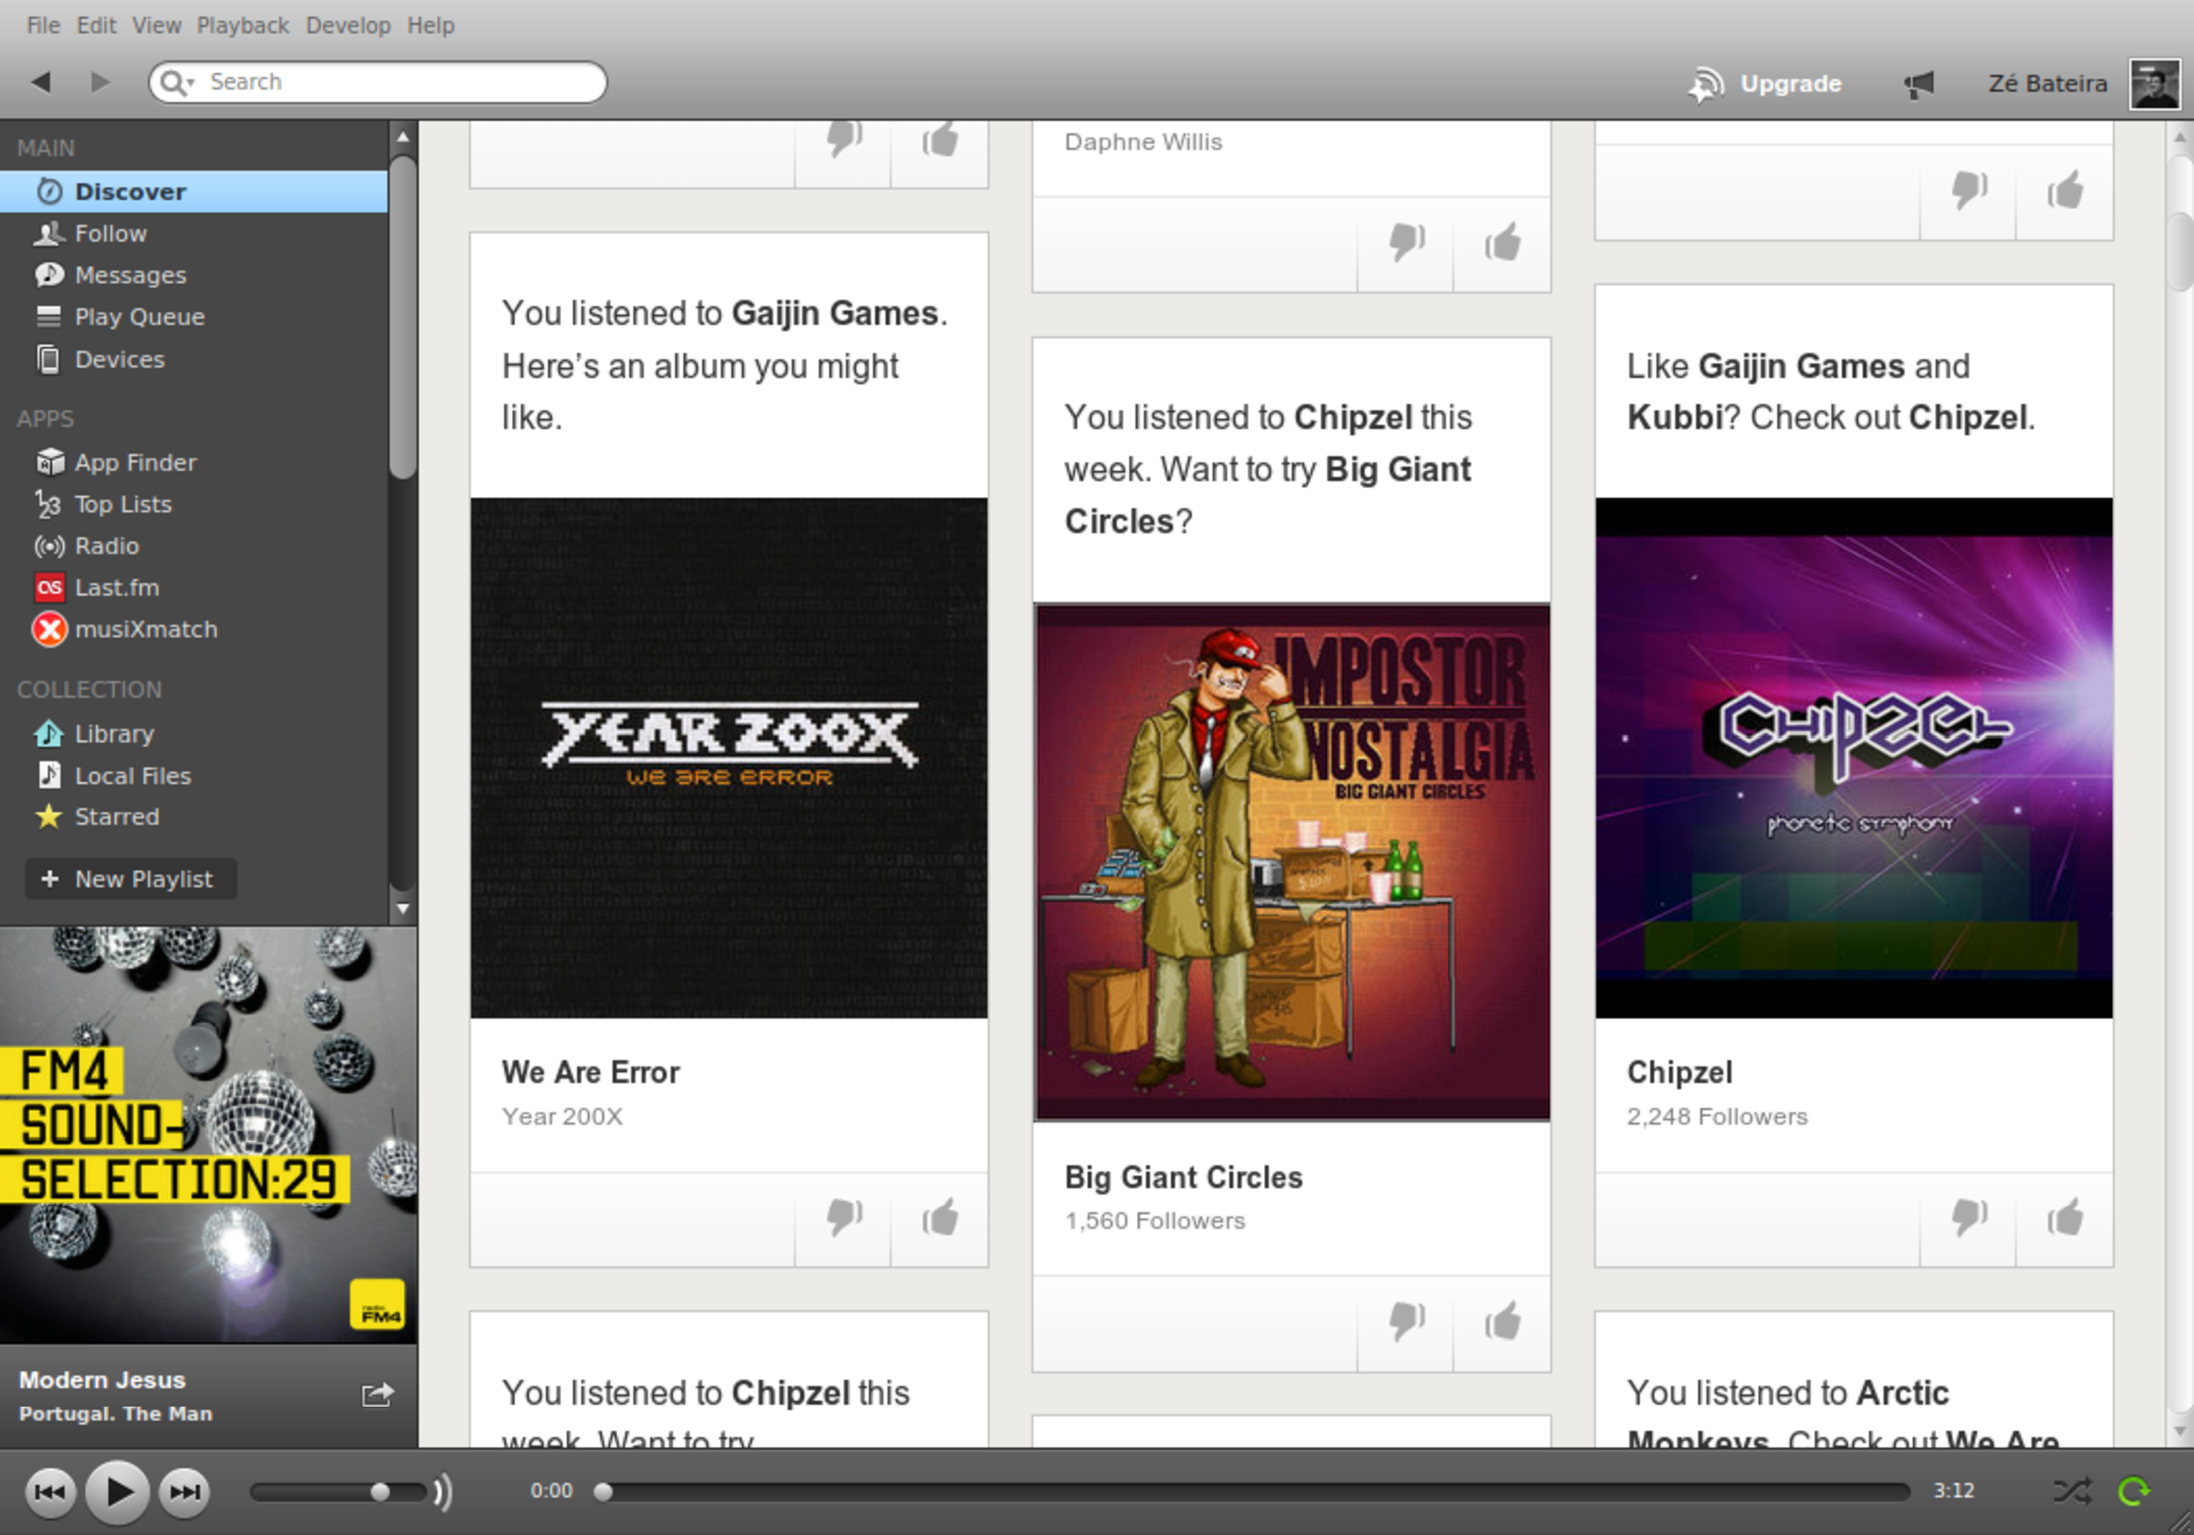
\includegraphics[width=\textwidth]{spotify.pdf}
        \end{center}
        \caption{Spotify: interface do modo de descoberta do \emph{desktop client}}
        \label{fig:spotify_apps}
      \end{figure}

      Na figura \ref{fig:spotify_apps} é possível ver o aspecto do \emph{Spotify Desktop Client}.
      É possível ver na barra lateral esquerda o \emph{App Finder}, dentro do separador \emph{Apps}, que permite ver quais as aplicações disponíveis e instalá-las com um clique.
 
      Na figura \ref{fig:spotify_apps2} está aberta a aplicação da Last.fm. É possível ver que as Aplicações Spotify têm apenas um espaço reservado embutido no \emph{Spotify Desktop Client}.

      \begin{figure}
        \begin{center}
          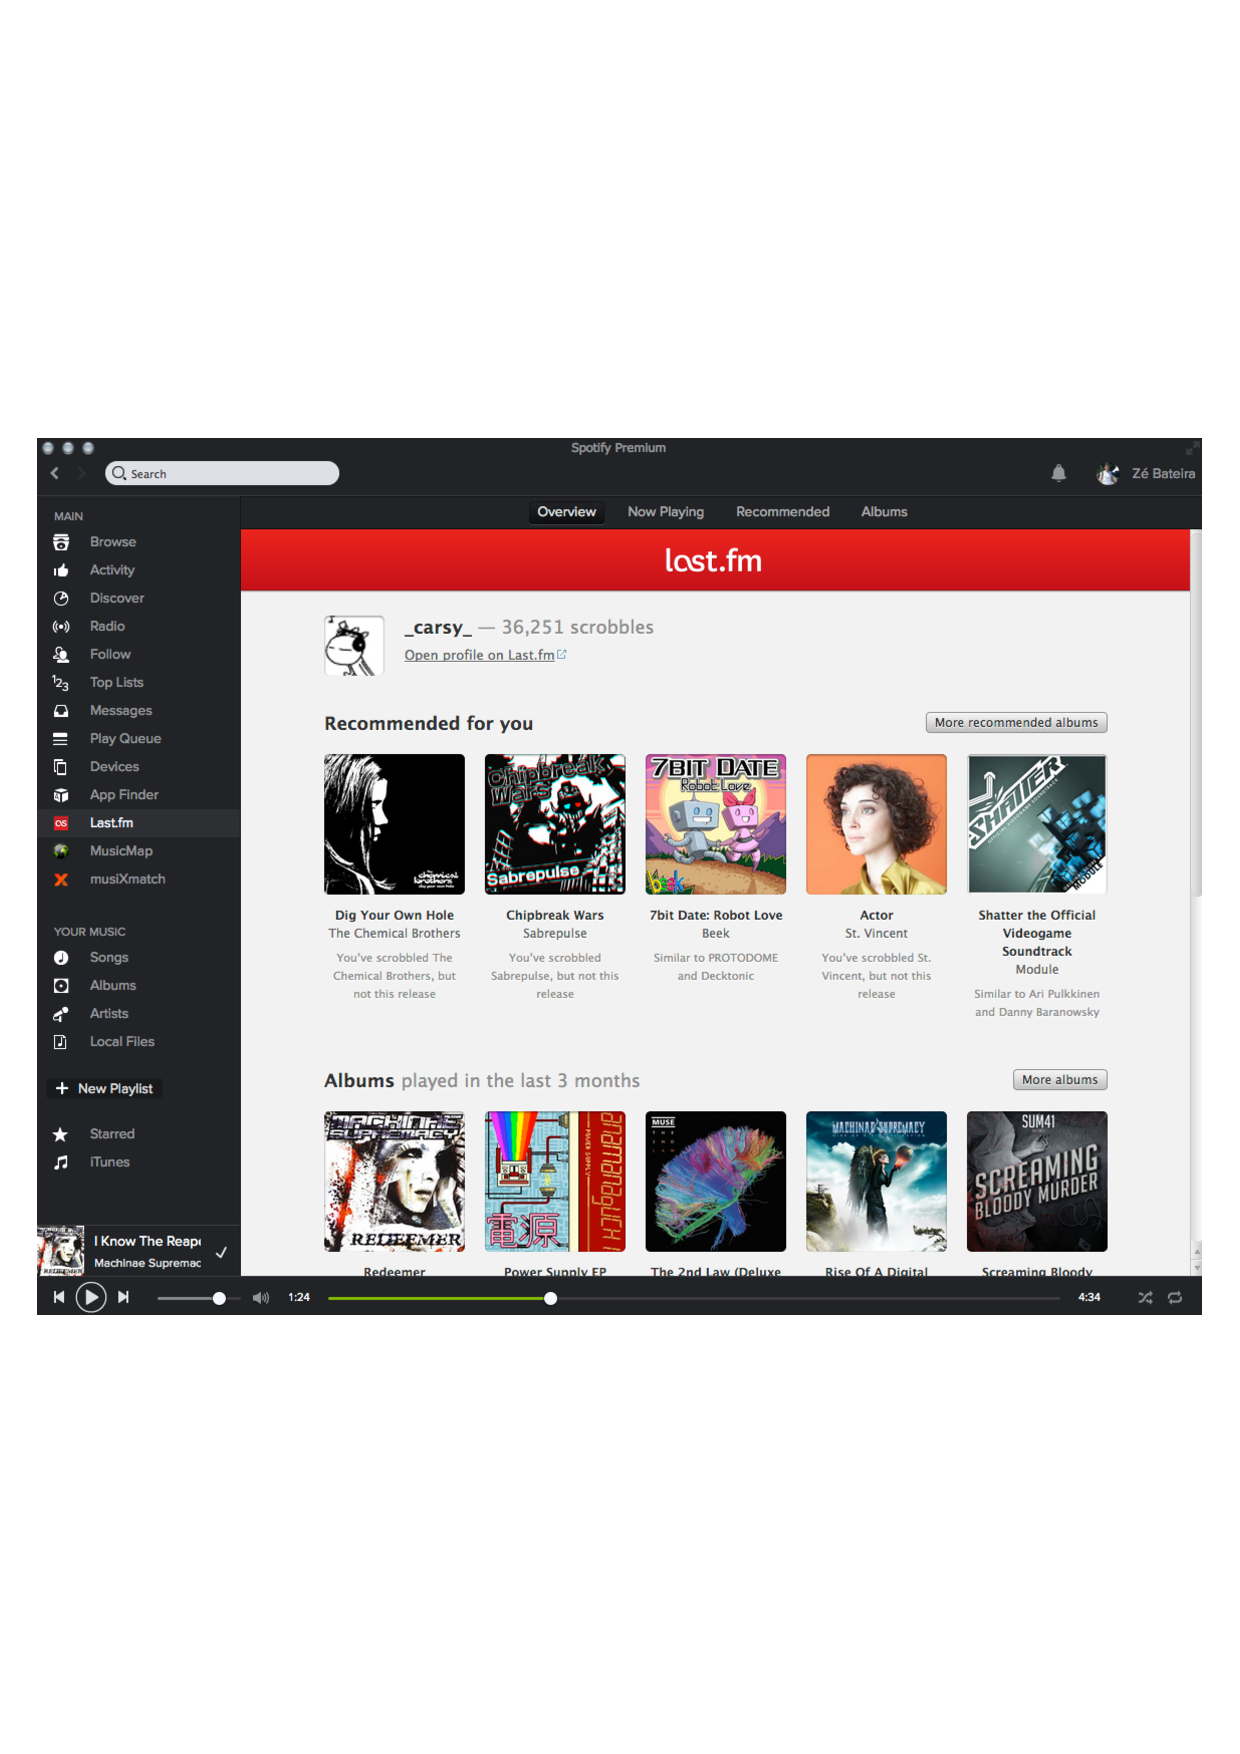
\includegraphics[width=\textwidth]{spotify_apps.pdf}
        \end{center}
        \caption{Spotify: Aplicação Last.fm aberta no \emph{Spotify Player}}
        \label{fig:spotify_apps2}
      \end{figure}


      
      Para o seu desenvolvimento destas aplicações são disponibilizadas duas \emph{frameworks}: \emph{API Framework}\footnote{https://developer.spotify.com/docs/apps/api/1.0/} e \emph{Views Framework}\footnote{https://developer.spotify.com/docs/apps/views/1.0/}.
      A primeira fornece uma interface para recolher metadados de artistas, álbuns e músicas e controlar o reprodutor de música.
      A segunda fornece componentes de design como botões, listas, abas, entre outros, para o desenvolvimento da aplicação.

      Para desenvolver os módulos \ref{item:obj4} e \ref{item:obj5} esta é a ferramenta mais apropriada.

    % subsubsection spotify_apps (end)


    \subsubsection{Spotify Widgets} % (fold)
    \label{ssub:spotify_widgets}
      As Widgets\footnote{https://developer.spotify.com/technologies/widgets} são pequenos componentes que se podem embeber em \emph{websites}.
      No momento da escrita deste relatório existem dois componentes: \emph{Play Button} e \emph{Follow Button}.

      No entanto, existe algumas limitações no uso destas componentes.
      No Spotify, apenas utilizadores que tenham criado conta no serviço Spotify é que podem usar o mesmo.
      O mesmo também se aplica a estas \emph{widgets} - apesar de estas existirem numa aplicação externa ao Spotify, apenas utilizadores Spotify podem usá-las.
      Esta limitação pode fazer sentido para o \emph{Follow Button}, mas o \emph{Play Button} torna-se inútil para utilizadores que não usem o Spotify.
      Outro problema surge quando a música do \emph{Play Button} não está disponível no País em que o utilizador está.

      Estas \emph{widgets} apenas servem de hiperligação ou ao \emph{Player} do Spotify ou ao \emph{WebPlayer} do Spotify.
      Na realidade, usando estas \emph{widgets}, o stream de música do Spotify é sempre reproduzido dentro do ambiente do Spotify, e nunca em aplicações externas.

      

    % subsubsection spotify_widgets (end)

    \subsubsection{Libspotify SDK} % (fold)
    \label{ssub:libspotify_sdk}
    
      Libspotify SDK\footnote{https://developer.spotify.com/technologies/libspotify} é uma API que permite adicionar os serviços do Spotify em aplicações externas.
      No entanto, existem algumas limitações para os utilizadores destas aplicações.

      
      Existem, dois tipos de conta a que o utilizador pode subscrever: conta grátis e conta \emph{premium}.
      Como foi referido anteriormente (\ref{ssub:spotify_widgets}) apenas utilizadores Spotify podem interagir com qualquer componente do Spotify, dentro ou fora das aplicações nativas do mesmo.
      Libspotify fornece uma interface que permite a um utilizador fazer \emph{login} no Spotify em aplicações externas por forma a poder ouvir música do Spotify, criar playlists e outras funcionalidades.
      No entanto, o único tipo de utilizadores que pode fazer \emph{login} nestas aplicações que usam Libspotify, são utilizadores \emph{premium}.

      Neste sentido, uma aplicação que, para funcionar, necessita de que o utilizador, para além de possuir uma conta Spotify, também pague uma subscrição mensal de utilizador premium, é uma aplicação bastante restritiva.

      Esta ferramenta pode ser usada para desenvolver o módulo \ref{item:obj6}.
      

    % subsubsection libspotify_sdk (end)


    \subsubsection{Metadata API} % (fold)
    \label{ssub:metadata_api}
    
      A \emph{Metadata API}\footnote{https://developer.spotify.com/technologies/web-api} disponibiliza publicamente informação de músicas, álbuns e artistas da Base de dados do Spotify.

      Através de pedidos HTTP

      ...




    % subsubsection metadata_api (end)

  % subsection ferramentas_de_desenvolvimento (end)

  \subsection{Experimentações Feitas} % (fold)
  \label{sub:experimentacoes}
  
    ...

  % subsection experimentacoes (end)

  \subsection{Conclusão} % (fold)
  \label{sub:conclusao}
  
    A escolha final do módulo a desenvolver é a Aplicação Spotify.

  % subsection conclusao (end)

% section spotify (end)

\section{Tecnologias} % (fold)
\label{sec:tecnologias}

  Tecnologias a serem usadas:

  \begin{description}
    \item[Spotify Desktop Client] \hfill \\
      O desenvolvimento de aplicações Spotify é feito de forma integrada no programa.
    \item[Webkit Development Tools - webkit.org] \hfill \\
      A aplicação do Spotify foi desenvolvida com Webkit, e por isso, as aplicações Spotify também o são.
    \item[Sublime Text - sublimetext.com] \hfill \\
      Um editor de texto bastante orientado a desenvolvimento web. Um dos mais usados neste contexto
    \item[Bower - bower.io] \hfill \\
      Gestor de pacotes de software e dependências orientado para desenvolvimento web
    \item[Gruntjs - gruntjs.com] \hfill \\
      Programa de gestão de tarefas automatizadas. Muito útil para testes, compilação e otimização de código
    \item[Arborjs - arborjs.org] \hfill \\
      Framework de javascript para desenho de grafos. Foi já utilizada no desenvolvimento do RAMA (existe sempre a possibilidade de se usar outra ferramenta substituta caso esta não for adequada)
  \end{description}

% section tecnologias (end)

\section{Arquitetura} % (fold)
\label{sec:arquitetura}

  Esquema geral da arquitetura da Aplicação.

% section arquitetura (end)

\section{Resumo e Conclusões}

  A escolha final do módulo a desenvolver é a Aplicação Spotify.
